\documentclass{article}

\usepackage[final,main]{neurips_2025}
\usepackage[utf8]{inputenc}
\usepackage[T1]{fontenc}
\usepackage{hyperref}
\usepackage{url}
\usepackage{array}
\usepackage{booktabs}
\usepackage{amsfonts}
\usepackage{amsmath}
\usepackage{graphicx}
\usepackage{microtype}

\makeatletter
\renewcommand{\@notice}{}
\makeatother

\title{Which Tasks Tell, Which Tools Help: IRT-Guided Agent Benchmarking}

\author{%
  Yiheng Yao\\
  Stanford University\\
  \texttt{yaoyh@stanford.edu}\\
}

\begin{document}

\maketitle

\begin{abstract}
Agent benchmarks usually report aggregate pass rates, but those scores hide large variation in which tasks distinguish strong and weak model--harness systems, and which tool affordances make those differences possible. This project treats agent benchmark outcomes as measurement data. Using response matrices from the Holistic Agent Leaderboard (HAL), we model binary task outcomes with multidimensional item response theory (IRT), estimate task difficulty and discrimination, and study whether trace-derived harness features explain systematic residual structure. The central question is whether a smaller high-information subset of tasks can preserve useful ranking and calibration signal while also revealing which harness tools help which models on which kinds of items.
\end{abstract}

\section{Introduction}

Modern agent evaluations are expensive because each new model--harness combination may require running hundreds or thousands of tasks. They are also statistically blunt: an aggregate benchmark score treats every item as equally informative, even though some tasks are solved by nearly every agent, some by almost none, and only a subset separates systems in ways that are useful for model selection or harness design. This creates two related measurement problems. First, we need to know which benchmark items carry high information about agent capability. Second, we need to know whether performance differences come from the base model, the harness, the benchmark domain, or interactions among models, tools, and task types.

The research question is: \emph{can IRT models fit to historical agent benchmark outcomes identify high-value tasks that preserve evaluation signal at lower cost, and can trace-derived harness features help explain which tools help which models on which kinds of items?}

Our approach differs from standard leaderboard analysis in three ways. First, we treat benchmark outcomes as a sparse item-response matrix rather than as aggregate pass rates. Second, we treat an evaluated agent as a model--harness system: the same base model may behave differently under different scaffolds, tools, prompts, and execution policies. Third, we use item-level residual structure to motivate tool and harness diagnostics, rather than assuming that benchmark-level labels such as ``SWE-bench'' or ``GAIA'' are sufficiently granular measurement units.

This project leverages the collected model $\times$ harness $\times$ benchmark dataset introduced by HAL \citep{hal2026}. The version analyzed here spans 59 recorded model labels and 68 recorded harness/scaffold labels, which we group into 20 semantic base-model groups and 15 semantic harness groups, across 10 benchmarks. Model-call settings such as reasoning effort are treated as model-configuration differences rather than separate harnesses. This normalization supports the paper's three analyses: item-level IRT for measurement, discrimination-based task downscaling for cheaper evaluation, and harness-aware residual analysis for generating targeted tool ablation hypotheses.

\begin{table}[t]
\centering
\small
\setlength{\tabcolsep}{4pt}
\begin{tabular}{lrrrrr}
\toprule
Benchmark & Tasks & Run configs & Norm. models & Norm. harnesses & Outcomes \\
\midrule
assistantbench & 33 & 33 & 10 & 2 & 1{,}089 \\
colbench\_backend\_programming & 1{,}000 & 10 & 7 & 1 & 10{,}000 \\
corebench\_hard & 45 & 66 & 17 & 3 & 2{,}970 \\
gaia & 165 & 37 & 13 & 2 & 6{,}104 \\
online\_mind2web & 336 & 36 & 12 & 2 & 10{,}800 \\
scicode & 65 & 38 & 11 & 3 & 2{,}470 \\
scienceagentbench & 102 & 25 & 12 & 2 & 2{,}550 \\
swebench\_verified\_mini & 50 & 45 & 15 & 2 & 2{,}147 \\
taubench\_airline & 50 & 47 & 12 & 3 & 2{,}334 \\
usaco & 307 & 15 & 10 & 2 & 4{,}605 \\
\bottomrule
\end{tabular}
\caption{Dataset coverage after regenerating the master binary outcome CSV and joining normalized metadata. The full matrix contains 45{,}069 observed outcomes across 10 benchmarks.}
\label{tab:dataset-coverage}
\end{table}

\section{Background and Related Work}

This project sits at the intersection of AI measurement science, item response theory, efficient evaluation, and process-level agent evaluation. Recent AI evaluation work argues that benchmarks should be understood as measurement instruments tied to explicit constructs and claims \citep{wallach2025socialmeasurement,salaudeen2025measurement,sun2025beyondbenchmarks}. We adopt that stance for agent harnesses: the target construct is not ``general intelligence,'' but the ability of model--harness systems to solve agentic benchmark items under particular tool affordances.

Item response theory was originally developed for educational testing, where the goal is to infer a respondent's latent ability from responses to items with varying difficulty and discrimination. The Rasch model and two-parameter logistic models provide a natural formalism for separating respondent ability from item difficulty and item informativeness \citep{rasch1960probabilistic,baker2001basics}. The same latent-variable view is closely related to probabilistic ranking models such as Bradley--Terry and Plackett--Luce models \citep{bradley1952rank,luce1959individual}, which infer strengths or utilities from noisy observations. In this project, agents replace students, benchmark tasks replace exam items, and binary pass/fail outcomes replace exam responses.

Recent LLM evaluation work has used IRT-style models to improve benchmark measurement and compression \citep{lalor2016evaluation,zhou2025lost}. Truong et al.'s amortized model-based evaluation uses related structure to predict benchmark performance from partial item responses \citep{truong2025amortized}. TinyBenchmarks similarly asks whether small curated subsets can recover full-benchmark estimates \citep{maiapolo2024tinybenchmarks}, while Zhang et al. caution that such prediction can fail when new frontier models differ from historical systems \citep{zhang2025missesmark}. This tension motivates our emphasis on held-out prediction, calibration, ranking stability, and cold-start evaluation.

Agentic benchmarks make the measurement problem sharper because final correctness is only one view of tool-using behavior. TRAJECT-Bench evaluates whether tools are selected, parameterized, and ordered correctly \citep{he2025traject}. AgentProcessBench provides human-labeled step annotations for tool-augmented trajectories \citep{fan2026agentprocessbench}. HAL addresses the complementary infrastructure problem by standardizing agent evaluation across models, scaffolds, and benchmarks \citep{hal2026}. Our contribution is the statistical measurement layer on top of such data: estimating which items are informative and whether harness/tool features explain model--item residual structure.

\section{Methods}

\begin{table}[!htbp]
\centering
\small
\begin{tabular}{lrrrr}
\toprule
Model terms & Features & Log loss & Pseudo-$R^2$ & AUC \\
\midrule
Benchmark & 10 & 0.536 & 0.111 & 0.674 \\
Benchmark + model + harness & 45 & 0.521 & 0.136 & 0.715 \\
+ model:harness + benchmark:harness & 232 & 0.513 & 0.150 & 0.733 \\
Task + model + harness & 2{,}188 & 0.361 & 0.401 & 0.905 \\
+ model:harness + benchmark:harness & 2{,}375 & 0.346 & 0.427 & 0.913 \\
+ task:harness & 5{,}618 & 0.331 & 0.451 & 0.920 \\
\bottomrule
\end{tabular}
\caption{Staged L2-regularized logistic audit. Pseudo-$R^2$ is McFadden-style deviance reduction relative to an intercept-only model. ``Task'' denotes task identity nested within benchmark.}
\label{tab:gstudy}
\end{table}

\paragraph{Data.}
The primary data source is constructed from HAL benchmark outcomes. We use ``agent configuration'' to mean an observed model--harness run configuration: conceptually a base model paired with a harness/scaffold, and operationally identified in the extracted data by model, scaffold, run id, and benchmark. The regenerated master binary outcome file, \texttt{irt\_data/response\_matrix.csv}, contains 45{,}069 observed responses from 352 such configurations, corresponding to 222 distinct raw model--scaffold pairs, 165 normalized model--harness pairs, 59 recorded model labels, 68 recorded harness/scaffold labels, and 2{,}153 benchmark-task pairs. Because some raw model and harness labels include provider names, model names, or reasoning settings, Appendix~\ref{app:dataset-inventory} reports the normalization from raw aliases to 20 semantic base-model groups and 15 semantic harness groups; reasoning effort is normalized onto the model-configuration side of the crossing rather than treated as a separate harness. Each row is an observed response $y_{ij} \in \{0,1\}$ for agent configuration $i$ on task $j$. The joinable metadata tables \texttt{irt\_data/model\_metadata.csv}, \texttt{irt\_data/harness\_metadata.csv}, and \texttt{irt\_data/harness\_affordances.csv} provide the canonical source of truth for normalized model labels, normalized harness labels, tool-exposure mechanisms, exposed-tool inventories, and binary harness affordance flags. Appendix~\ref{app:tool-exposure-taxonomy} defines the tool-passage taxonomy, records the exposed tools for each normalized harness, and explains how the affordance flags are generated from harness source, configuration, and trace metadata.

\subsection{Pseudo G-Study: Measurement Design Audit}

Before fitting IRT, we run a lightweight generalizability-theory-inspired audit to decide where the measurement model needs resolution. The HAL matrix is sparse and unbalanced, and full crossed Bernoulli mixed models with high-cardinality interactions were computationally unstable. We therefore fit staged L2-regularized logistic models and compare McFadden-style pseudo-$R^2$, deviance, AUC, and residual structure (details in Appendix~\ref{app:pseudo-gstudy}):
\[
\begin{aligned}
  y &\sim \text{benchmark} + \text{model} + \text{harness}
       + \text{model}:\text{harness}
       + \text{benchmark}:\text{harness},\\
  y &\sim \text{task}(\text{benchmark}) + \text{model} + \text{harness}
       + \text{model}:\text{harness}
       + \text{benchmark}:\text{harness},\\
  y &\sim \text{task}(\text{benchmark}) + \text{model} + \text{harness}
       + \text{task}:\text{harness}.
\end{aligned}
\]
This audit is not a causal tool analysis and does not estimate literal Gaussian variance components. It is a likelihood-based measurement diagnostic. If task identity and harness interactions materially reduce Bernoulli deviance, then aggregate benchmark scores are too coarse, and the subsequent model should be item-level and harness-aware.

\subsection{Multidimensional IRT Model}

The main model is a multidimensional two-parameter IRT model:
\[
  P(y_{ij}=1) = \sigma(\theta_i^\top a_j + d_j),
\]
where $\theta_i \in \mathbb{R}^K$ is the latent ability vector of agent configuration $i$, $a_j \in \mathbb{R}^K$ is the discrimination vector for task $j$, $d_j$ is task easiness, and $\sigma$ is the logistic function. We train by minimizing binary cross-entropy over observed agent--task outcomes. We sweep small values of $K$ and compare latent-only models against feature-informed models in which agent and task metadata are projected into the same $K$-dimensional space and added to the learned latent embeddings. The fitted model supports two co-equal analyses: task discrimination for reducing benchmark size, and residual structure for identifying model--harness and harness--task interactions.

\subsection{Harness Feature and Residual Model}

The feature-informed model decomposes each agent configuration into model, harness, and task features. Model features include provider, normalized model family, and model-call configuration metadata such as reasoning effort where available. Harness features come from the normalized taxonomy in Appendix~\ref{app:tool-exposure-taxonomy}: a categorical tool-passage mechanism, a concrete exposed-tool inventory, and binary affordance flags for code generation, code execution, shell access, file read/edit, web search, page browsing, browser control, vision, native domain tools, benchmark API tools, human dialogue, retrieval context, external judging/evaluation, self-debug feedback, and complete-program prompting. Task features include benchmark domain and coarse task type.

We use these features in two ways. First, in the feature-informed IRT model, metadata provides a cold-start prior for configurations with weak or absent response history. We distinguish three cold-start information regimes: \emph{different-harness}, where the model is known but evaluated through a harness not observed with that model in the benchmark; \emph{open-code}, where source/configuration inspection gives harness affordance flags before any outcomes are observed; and \emph{partially open-trace}, where a small trace subsample is available to refine affordance labels before predicting the remaining tasks. Second, after fitting the IRT model, we compute response residuals $r_{ij}=y_{ij}-\hat p_{ij}$ and aggregate them by normalized model family, harness, benchmark/task type, and affordance flags. This residual analysis asks whether particular tool-passage mechanisms or affordances are associated with systematic over- or under-performance after accounting for item difficulty and overall agent ability. These estimates are observational and hypothesis-generating: tool exposure is confounded with many harness design choices, and exposure does not guarantee effective tool use.

\subsection{Task Selection and Adaptive Evaluation}

After fitting the model, we rank tasks by discrimination magnitude $\|a_j\|$ within each benchmark. We construct fixed subsets that cover 50\%, 70\%, 80\%, and 90\% of total estimated discrimination mass. These subsets operationalize the question: how much of the benchmark's agent-separating signal can be preserved with fewer tasks? This connects the IRT model to active learning and sample-efficient measurement: the fixed subsets are a static approximation to adaptive testing policies that would select high-information items as evidence accumulates.

\subsection{Evaluation Protocol}

We evaluate predictive and ranking quality on a reproducible semantic holdout split. The leakage unit is benchmark $\times$ normalized model $\times$ normalized harness, since a row-level random split would place the same semantic model--harness unit in both train and test through raw aliases or repeated runs. For each benchmark $\times$ normalized harness cell, the split holds out one representative normalized model whose pass rate is closest to that cell's median, avoiding obvious cherry-picking of only unusually strong or weak systems. The resulting split contains 39{,}461 training rows and 5{,}608 holdout rows, with no leakage-unit overlap between train and holdout.

Metrics include binary cross-entropy, AUC, accuracy, Brier score, calibration error, rank correlation between full-suite and subset-based agent rankings, and stability of selected high-discrimination tasks under resampling. For the feature analysis, we compare latent-only and metadata-informed models on held-out semantic units. For cost-aware evaluation, we report task-count reduction at each discrimination-coverage threshold and the loss in predictive or ranking fidelity relative to the full benchmark.

\section{Results and Discussion}

\subsection{Exploratory Measurement Audit}

Table~\ref{tab:gstudy} reports the pseudo G-study on the regenerated 45{,}069-row response matrix. Benchmark labels alone reduce Bernoulli deviance only modestly relative to the intercept-only model ($R^2_{\mathrm{pseudo}}=0.111$). Adding normalized model and harness main effects raises this to 0.136, while model--harness compatibility raises it to 0.150. In contrast, replacing benchmark identity with task identity nested within benchmark produces a much larger jump ($R^2_{\mathrm{pseudo}}=0.401$). Adding model--harness and benchmark--harness interactions reaches 0.427, and a task--harness term reaches 0.451. This supports the paper's central modeling choice: benchmark-level aggregation is too coarse, and the useful resolution is item-level and harness-aware.

The regularized interaction coefficients also provide an initial qualitative check that harness effects are not scalar. HF Open Deep Research shows positive model--harness residual structure with GPT-5, o4-mini, GPT-4.1, and Claude Opus 4, but negative residual structure with Claude Opus 4.1 and Claude Sonnet 4.5. HAL Generalist shows the complementary pattern of stronger residual performance with several Claude-family configurations and weaker residual performance with o3, Gemini, and DeepSeek variants. These are descriptive in-sample diagnostics, not causal tool effects, but they motivate the later held-out MIRT residual analysis of which harness mechanisms fit which model families and item types.

\subsection{MIRT Model Comparison}

Table~\ref{tab:mirt-sweep} reports the semantic-holdout sweep. Because all
holdout agent configurations are unseen under the split unit, latent-only
models cannot estimate a held-out agent ability vector from response history.
For this evaluation, unseen latent-only agents are scored with zero
$\theta_i$, so their predictions reduce mostly to task easiness. The
feature-informed models also zero unseen learned embeddings, but retain the
metadata projection $f_{\mathrm{agent}}(x_i)$, giving a genuine cold-start
agent vector without fitting on held-out responses. Feature-informed models
therefore dominate latent-only models on holdout BCE and Brier score. The
$K=2$ feature-informed model is the best prediction model by holdout AUC,
while the $K=1$ feature-informed model gives the strongest
benchmark-compression operating point.

\begin{table}[t]
\centering
\small
\begin{tabular}{rr rrrrr}
\toprule
$K$ & Features & BCE & AUC & Accuracy & Brier & Cal. error \\
\midrule
1 & yes & 0.358 & 0.895 & 0.835 & 0.113 & 0.030 \\
2 & yes & 0.362 & 0.900 & 0.833 & 0.116 & 0.086 \\
4 & yes & 0.376 & 0.896 & 0.832 & 0.117 & 0.072 \\
8 & yes & 0.425 & 0.890 & 0.821 & 0.129 & 0.124 \\
1 & no & 0.566 & 0.861 & 0.823 & 0.188 & 0.191 \\
2 & no & 0.583 & 0.852 & 0.827 & 0.196 & 0.184 \\
4 & no & 0.596 & 0.844 & 0.823 & 0.202 & 0.195 \\
8 & no & 0.604 & 0.842 & 0.825 & 0.206 & 0.228 \\
\bottomrule
\end{tabular}
\caption{Holdout performance on the split-v1 semantic holdout. The leakage
unit is benchmark $\times$ normalized model $\times$ normalized harness. Lower
BCE, Brier, and calibration error are better; higher AUC and accuracy are
better.}
\label{tab:mirt-sweep}
\end{table}

There is also a prediction--reduction tradeoff across fitted models. At the
80\% discrimination-coverage threshold, the $K=2$ feature-informed model has
the best holdout AUC (0.900) but removes only 20.6\% of tasks on average.
The $K=1$ feature-informed model has slightly lower AUC (0.895) and the best
holdout BCE (0.358), but its discrimination mass is more concentrated: it
removes 46.2\% of tasks on average at the same 80\% coverage threshold.
Thus the Pareto frontier contains at least two useful operating points: $K=2$
for maximum ranking signal, and $K=1$ for a more aggressive screening subset
with only a small AUC loss.

\begin{figure}[t]
\centering
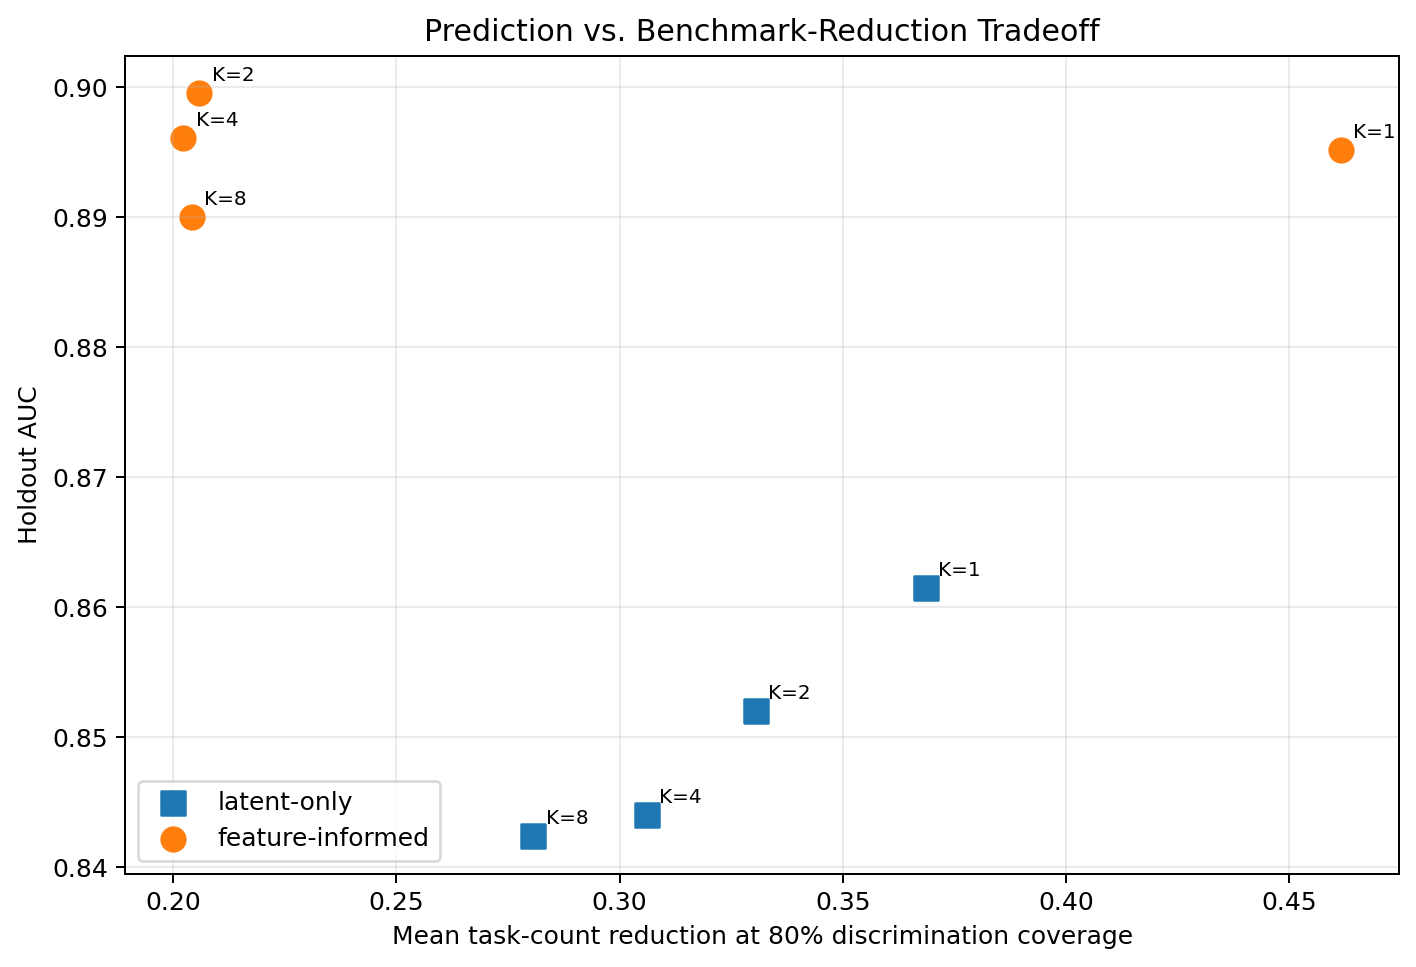
\includegraphics[width=0.82\linewidth]{figures/split_v1_auc_reduction_tradeoff.png}
\caption{Tradeoff between holdout AUC and mean task-count reduction at the
80\% discrimination-coverage threshold. Feature-informed $K=1$ and $K=2$
models form the useful frontier: $K=2$ maximizes AUC, while $K=1$ gives much
larger task reduction with a small AUC decrease.}
\label{fig:auc-reduction-tradeoff}
\end{figure}

\subsection{Benchmark Downscaling}

Using the compression-oriented $K=1$ feature-informed model, we rank tasks
within each benchmark by $|a_j|$ and compute the number of tasks needed to
retain fixed fractions of total discrimination mass.
Figure~\ref{fig:cost-reduction} shows the resulting downscaling curves.
The fitted one-dimensional discrimination spectrum is substantially more
concentrated than the higher-dimensional spectra: retaining 80\% of
discrimination mass keeps a mean of 53.8\% of tasks across benchmarks,
corresponding to a mean 46.2\% task-count reduction. At 70\% discrimination
coverage, the mean task-count reduction is 55.6\%; at 90\% coverage, it is
32.1\%. In aggregate task-count terms, the conservative 90\% threshold retains
1{,}426 of 2{,}153 tasks and removes 727 tasks, corresponding to a 33.8\%
estimated benchmark-cost reduction. This gives the strongest screening
contribution: the $K=1$ feature model gives up only 0.004 holdout AUC relative
to $K=2$ with features while cutting nearly half of benchmark tasks at the
80\% discrimination threshold and roughly one-third of tasks even at the
conservative 90\% threshold.

\begin{figure}[t]
\centering
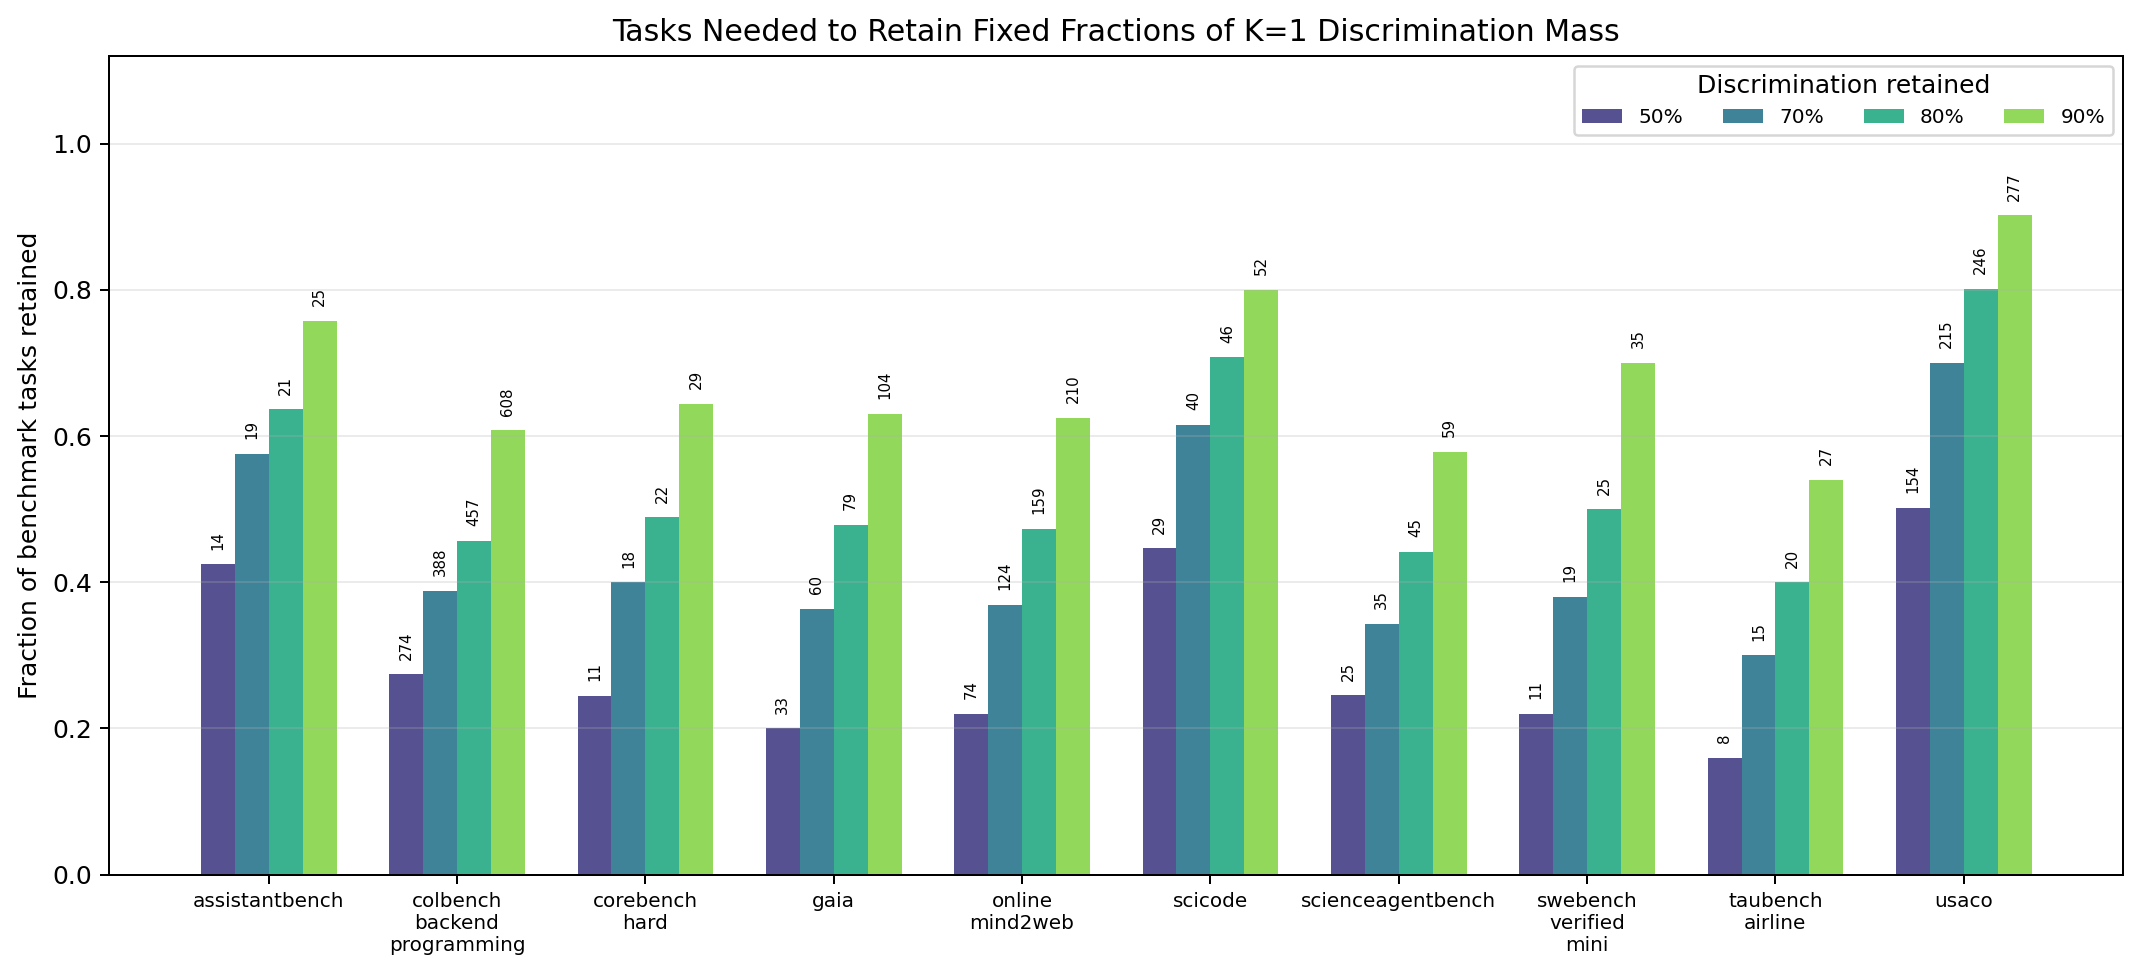
\includegraphics[width=\linewidth]{figures/split_v1_k1_features_cost_reduction.png}
\caption{Fraction of tasks retained to preserve fixed fractions of total
estimated discrimination mass under the compression-oriented $K=1$
feature-informed MIRT model. Bar labels give the retained task count.}
\label{fig:cost-reduction}
\end{figure}

\subsection{Which Tool Interfaces Help?}

The strongest tool result is a negative one: broad code-agent tool registries
often underperform benchmark-specialized interfaces in matched comparisons.
Table~\ref{tab:harness-contrasts} reports same-benchmark, same-model contrasts
where the base model is held fixed and only the harness/tool interface changes.
On SWE-bench, SWE-Agent's repository workflow---file-map navigation, shell and
editor commands, diff/review state, and explicit submit actions---substantially
outperforms HAL Generalist's code-agent registry for every shared model shown.
On TAU-bench Airline, native airline tool schemas outperform HAL Generalist's
wrapped domain actions. On ScienceAgentBench, SAB Self-Debug outperforms HAL
Generalist for the shared o3 run, suggesting that complete-program generation
plus harness execution/debug feedback is better aligned with scientific coding
tasks than a general-purpose registry loop.

\begin{table}[t]
\centering
\footnotesize
\setlength{\tabcolsep}{3pt}
\begin{tabular}{ll>{\raggedright\arraybackslash}p{1.45in}rrr}
\toprule
Benchmark & Model & Interface contrast & Task-specific & HAL registry & $\Delta$ \\
\midrule
SWE-bench & o3 & SWE-Agent vs. HAL Generalist & 0.593 & 0.000 & 0.593 \\
SWE-bench & o4-mini & SWE-Agent vs. HAL Generalist & 0.551 & 0.040 & 0.511 \\
SWE-bench & GPT-5 & SWE-Agent vs. HAL Generalist & 0.640 & 0.140 & 0.500 \\
SWE-bench & GPT-4.1 & SWE-Agent vs. HAL Generalist & 0.469 & 0.020 & 0.449 \\
TAU-bench & GPT-4.1 & TAU FewShot vs. HAL Generalist & 0.560 & 0.160 & 0.400 \\
TAU-bench & o4-mini & TAU FewShot vs. HAL Generalist & 0.545 & 0.200 & 0.345 \\
TAU-bench & o3 & TAU ToolCalling vs. HAL Generalist & 0.540 & 0.208 & 0.332 \\
ScienceAgentBench & o3 & SAB Self-Debug vs. HAL Generalist & 0.333 & 0.098 & 0.235 \\
\bottomrule
\end{tabular}
\caption{Matched same-model, same-benchmark pass-rate contrasts.
``Task-specific'' means the benchmark-specialized interface, which may be a
repo-repair workflow, native domain-tool schema, or execution/debug scaffold.
``HAL registry'' is HAL Generalist's code-agent tool registry. These
observational contrasts motivate targeted ablations; they do not by themselves
identify causal effects of individual tools.}
\label{tab:harness-contrasts}
\end{table}

The pattern suggests that ``which tools help'' is conditional on the task's
latent work loop. Repository-editing affordances help software repair, native
domain schemas help transactional customer-service tasks, and execution/debug
feedback helps scientific coding. Conversely, simply exposing many tools
through a broad code-agent registry is not enough: the interface must make the
task-relevant workflow easy for the model to represent and execute.
A targeted tool-count check supports this interpretation: across matched
benchmark $\times$ normalized-model configurations, the lower-tool-count
harness wins 61.7\% of comparisons, but the largest counterexamples are
task-aligned native schemas such as TAU-bench.
Appendix~\ref{app:swebench-trace-audit} audits matched SWE-bench traces and
shows that HAL Generalist does have live execution and edit affordances; the
stark SWE-bench gap therefore motivates interface-level ablations rather than a
simple sandbox/no-sandbox explanation.

\paragraph{Model--harness heatmap.}
Figure~\ref{fig:cold-start-heatmap} shows the demo heatmap view for SWE-bench Verified Mini, aggregating outcomes by normalized model and harness. Green cells are observed accuracies; blue italic cells are IRT cold-start predictions for model--harness pairs without observed runs in that benchmark slice. The view makes the main qualitative pattern visible: SWE-Agent's repository-specific workflow dominates the broad HAL Generalist registry on shared models, while the SAB Self-Debug column is an extrapolated prediction rather than a measured SWE-bench result.

\begin{figure}[t]
\centering
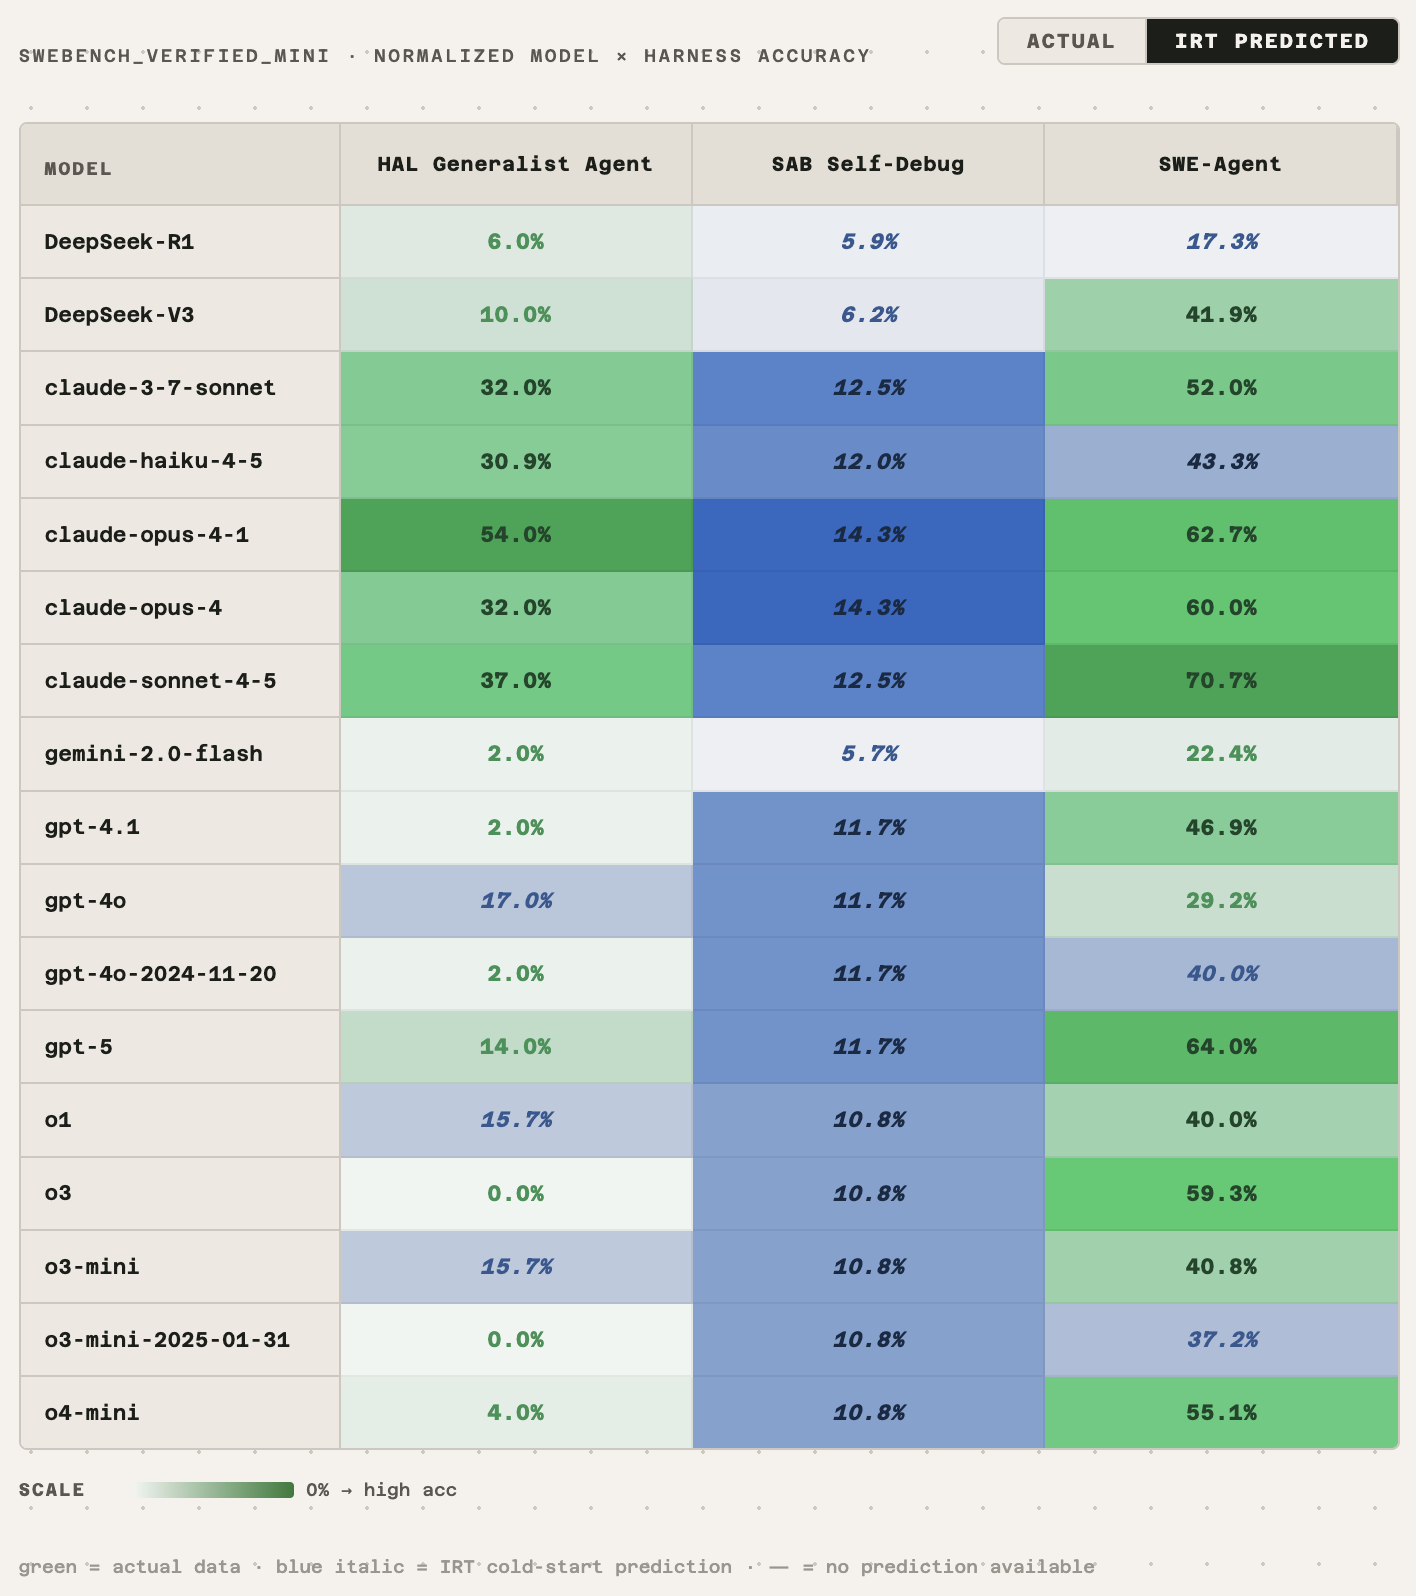
\includegraphics[width=0.88\linewidth]{figures/swebench_verified_mini_accuracy_demo_heatmap.png}
\caption{Demo heatmap for SWE-bench Verified Mini accuracy by normalized model and harness. Green cells are observed pass rates; blue italic cells are IRT cold-start predictions for unobserved model--harness combinations.}
\label{fig:cold-start-heatmap}
\end{figure}

\paragraph{Targeted ablation hypotheses.}
These contrasts suggest three concrete small-budget ablations: pass TAU-bench
native schemas directly through HAL Generalist rather than through registry
wrappers; add a SWE-Agent-like file-map/edit/review loop to HAL Generalist on
SWE-bench, or disable pieces of that loop inside SWE-Agent; and run SAB with
self-debug feedback disabled to separate complete-program prompting from
execution-loop feedback. The goal is not to exhaustively optimize a harness,
but to test whether the measurement model produces plausible interventions.

\paragraph{Limitations.}
The main limitations are sparsity, benchmark heterogeneity, non-random tool exposure, and dependence on the semantic split. A harness may expose a tool without using it well; conversely, a missing tool may proxy for many other scaffold design choices. The holdout split tests generalization across benchmark-specific model--harness units, but it does not prove performance on entirely unseen future models or unseen harnesses. We therefore treat tool-feature estimates as hypothesis-generating and rely on targeted ablations for stronger evidence.

\newpage
\section{Conclusion}

HAL outcomes are more informative when modeled as item-response data for model--harness systems than when reduced to aggregate leaderboard scores. In the 45{,}069-row matrix, task identity and task--harness interactions explain far more deviance than benchmark labels alone, motivating item-level IRT. On the semantic holdout, feature-informed MIRT gives a cold-start gain over latent-only models: $K=2$ with features is the best prediction setting (AUC 0.900), while $K=1$ with features is the best screening setting. At a conservative 90\% discrimination-mass threshold it removes 727 of 2{,}153 tasks, a 33.8\% aggregate cost reduction; at 80\% it removes nearly half of tasks on average. The tool analysis points to a conditional answer to ``which tools help'': specialized, task-aligned interfaces---repository editing for SWE-bench, native schemas for TAU-bench, and execution/debug feedback for scientific coding---beat a broad code-agent registry in matched comparisons. The resulting ablation agenda is concrete: test native-schema passthrough, repo-workflow components, and self-debug feedback as targeted interventions rather than treating tool exposure as a monolithic capability.

\bibliographystyle{plainnat}
\bibliography{references}

\appendix
\section{Pseudo G-Study Methodology}
\label{app:pseudo-gstudy}

Classical generalizability theory decomposes measurement variation across facets such as persons, items, raters, and occasions. In HAL, the analogous facets are base model, harness, benchmark, and task. A balanced random-effects G-study is not appropriate because the observed response matrix is sparse and highly unbalanced: not every model--harness pair is evaluated on every task.

We initially considered Bernoulli mixed-effects models of the form
\[
\begin{aligned}
y \sim 1
    &+ (1|\text{task}) + (1|\text{model}) + (1|\text{harness})\\
    &+ (1|\text{model}:\text{harness})
     + (1|\text{benchmark}:\text{harness})
     + (1|\text{task}:\text{harness}).
\end{aligned}
\]
This is the closest analogue to a G-study for binary outcomes, but the full Bayesian version was computationally unstable for the current matrix, especially with high-cardinality task--harness effects. We therefore use a staged L2-regularized logistic fixed-effect audit in the main analysis.

For each staged model, we compute Bernoulli log loss,
\[
\ell = -\frac{1}{N}\sum_i \left[y_i\log p_i + (1-y_i)\log(1-p_i)\right],
\]
and deviance,
\[
D = 2N\ell.
\]
We report McFadden-style pseudo-$R^2$,
\[
R^2_{\mathrm{pseudo}} = 1 - \frac{D_{\mathrm{model}}}{D_{\mathrm{null}}},
\]
where the null model is intercept-only. This quantity should be interpreted as relative reduction in Bernoulli deviance, not as ordinary least-squares variance explained. Because all staged models are fit to the same binary rows and likelihood family, the comparisons indicate which facets materially reduce predictive uncertainty.

We do not use a Gaussian linear mixed model as the main audit because the outcome is binary. A linear probability mixed model can produce probabilities outside $[0,1]$, has heteroskedastic residuals by construction, and estimates variance components on a scale that does not match the Bernoulli likelihood used by the IRT model. The staged logistic audit is therefore a more regular and reproducible diagnostic for this response matrix.

\section{Dataset Inventory}
\label{app:dataset-inventory}

This appendix groups the benchmark, model, and harness/scaffold labels present in the regenerated training response matrix. The raw HAL metadata contains provider prefixes, date suffixes, reasoning-setting suffixes, and model names embedded in some harness labels. For modeling, we therefore treat the raw labels as aliases and normalize them into semantic model and harness groups. This is especially important for harnesses: labels such as ``Core Agent Opus 4.5'' describe a CORE-Agent run paired with a particular model, not a fundamentally separate harness. Likewise, ``HAL Generalist High Reasoning'' is normalized as the HAL Generalist harness paired with a model configuration that sets a reasoning/thinking budget.

\subsection{Benchmarks}

\begin{table}[h]
\centering
\small
\begin{tabular}{>{\raggedright\arraybackslash}p{0.34\linewidth}>{\raggedright\arraybackslash}p{0.58\linewidth}}
\toprule
Benchmark & Brief description \\
\midrule
assistantbench & Assistant-oriented web and information-seeking tasks evaluated with browser-capable agents. \\
colbench\_backend\_programming & Backend programming tasks from ColBench. \\
corebench\_hard & Hard CORE-Bench tasks emphasizing complex tool-using problem solving. \\
gaia & General Assistant benchmark tasks requiring multi-step reasoning and external information use. \\
online\_mind2web & Web navigation and interaction tasks derived from Mind2Web-style environments. \\
scicode & Scientific coding tasks requiring code synthesis and problem-specific reasoning. \\
scienceagentbench & ScienceAgentBench tasks evaluating scientific analysis and self-debugging workflows. \\
swebench\_verified\_mini & A compact verified SWE-bench subset for software-engineering issue resolution. \\
taubench\_airline & TAU-bench airline customer-service tool-use tasks. \\
usaco & Competitive-programming tasks from the USACO-style coding environment. \\
\bottomrule
\end{tabular}
\caption{Benchmarks represented in the regenerated response matrix.}
\end{table}

\subsection{Semantic Model and Model-Configuration Groups}

The 59 recorded model labels collapse to 20 semantic base-model groups. When a run sets reasoning\_effort or an equivalent provider reasoning-token budget, we treat that as part of the model configuration rather than as a separate harness. Thus, for example, gpt-5 with high reasoning effort and gpt-5 with minimal reasoning effort are distinct model configurations paired with the same HAL Generalist harness. We keep the raw aliases visible so that the normalization remains auditable. The joinable model normalization table used for analysis is stored in \texttt{irt\_data/model\_metadata.csv}; it preserves each raw model label while recording the normalized base-model group and provider/family metadata.

\begingroup
\footnotesize
\begin{itemize}
\item \textbf{Claude 3.7 Sonnet}: Anthropic Claude Sonnet model. Aliases: anthropic/claude-3-7-sonnet-20250219; anthropic/claude-3.7-sonnet; claude-3-7-sonnet-20250219; openrouter/anthropic/claude-3.7-sonnet; openrouter/anthropic/claude-3.7-sonnet:thinking.
\item \textbf{Claude Haiku 4.5}: Anthropic Claude Haiku model. Aliases: anthropic/claude-haiku-4-5; claude-haiku-4-5; claude-haiku-4-5-20251001; openrouter/anthropic/claude-haiku-4.5.
\item \textbf{Claude Opus 4}: Anthropic Claude Opus model. Aliases: claude-opus-4-20250514; openrouter/anthropic/claude-opus-4.
\item \textbf{Claude Opus 4.1}: Anthropic Claude Opus model. Aliases: anthropic/claude-opus-4.1; claude-opus-4-1; claude-opus-4-1-20250805; openrouter/anthropic/claude-opus-4.1.
\item \textbf{Claude Opus 4.5}: Anthropic Claude Opus model. Aliases: anthropic/claude-opus-4-5-20251101; claude-opus-4-5; claude-opus-4-5-20251101.
\item \textbf{Claude Sonnet 4}: Anthropic Claude Sonnet model. Alias: claude-sonnet-4-20250514.
\item \textbf{Claude Sonnet 4.5}: Anthropic Claude Sonnet model. Aliases: anthropic/claude-sonnet-4-5; anthropic/claude-sonnet-4-5-20250929; claude-sonnet-4-5; claude-sonnet-4-5-20250929; openrouter/anthropic/claude-sonnet-4.5.
\item \textbf{DeepSeek R1}: DeepSeek reasoning model. Aliases: deepseek-ai/DeepSeek-R1; deepseek/deepseek-r1; openrouter/deepseek/deepseek-r1; openrouter/deepseek/deepseek-r1-0528; together\_ai/deepseek-ai/DeepSeek-R1.
\item \textbf{DeepSeek V3 / Chat}: DeepSeek chat model family. Aliases: deepseek-ai/DeepSeek-V3; deepseek/deepseek-chat; openrouter/deepseek/deepseek-chat-v3-0324; openrouter/deepseek/deepseek-chat-v3.1; together\_ai/deepseek-ai/DeepSeek-V3.
\item \textbf{Gemini 2.0 Flash}: Google Gemini Flash model. Aliases: gemini-2.0-flash; gemini/gemini-2.0-flash; google/gemini-2.0-flash-001.
\item \textbf{Gemini 2.5 Pro Preview}: Google Gemini Pro preview model. Aliases: gemini-2.5-pro-preview-03-25; gemini/gemini-2.5-pro-preview-03-25.
\item \textbf{Gemini 3 Pro Preview}: Google Gemini Pro preview model. Alias: google/gemini-3-pro-preview.
\item \textbf{GPT-4.1}: OpenAI GPT-4.1 model. Aliases: gpt-4.1; gpt-4.1-2025-04-14; openai/gpt-4.1-2025-04-14.
\item \textbf{GPT-4o}: OpenAI GPT-4o model. Aliases: gpt-4o; gpt-4o-2024-11-20.
\item \textbf{GPT-5}: OpenAI GPT-5 model. Aliases: gpt-5; gpt-5-2025-08-07; openai/gpt-5; openai/gpt-5-2025-08-07.
\item \textbf{GPT-OSS 120B}: OpenAI open-weight GPT-OSS model. Alias: openrouter/openai/gpt-oss-120b.
\item \textbf{o1}: OpenAI reasoning model. Alias: o1.
\item \textbf{o3}: OpenAI reasoning model. Aliases: o3-2025-04-03; o3-2025-04-16; openai/o3-2025-04-16.
\item \textbf{o3-mini}: OpenAI smaller reasoning model. Aliases: o3-mini; o3-mini-2025-01-31; openai/o3-mini-2025-01-31.
\item \textbf{o4-mini}: OpenAI smaller reasoning model. Aliases: o4-mini-2025-04-16; openai/o4-mini-2025-04-16.
\end{itemize}
\endgroup

\subsection{Reasoning-Effort Normalization}

Reasoning-effort labels in raw run names are normalized onto the model-configuration side. For direct providers that support the parameter, HAL Generalist passes reasoning\_effort to the model call. For OpenRouter-backed runs, the same setting is mapped to a reasoning-token budget. The normalized harness remains unchanged.

\begin{table}[h]
\centering
\small
\begin{tabular}{>{\raggedright\arraybackslash}p{0.36\linewidth}>{\raggedright\arraybackslash}p{0.24\linewidth}>{\raggedright\arraybackslash}p{0.30\linewidth}}
\toprule
Raw label pattern & Normalized harness & Normalized model configuration \\
\midrule
HAL Generalist High Reasoning with gpt-5 & HAL Generalist & GPT-5 with high reasoning effort \\
HAL Generalist Minimal Reasoning with gpt-5 & HAL Generalist & GPT-5 with minimal reasoning effort \\
HAL Generalist No Reasoning with Claude Opus 4.1 & HAL Generalist & Claude Opus 4.1 with no explicit reasoning budget \\
HAL Generalist Agent o4-mini high/low & HAL Generalist & o4-mini with high/low reasoning effort \\
HAL Generalist Agent o3 medium & HAL Generalist & o3 with medium reasoning effort \\
\bottomrule
\end{tabular}
\caption{Examples of reasoning-effort normalization. Reasoning settings are treated as model-call configuration, not as different HAL Generalist harnesses.}
\end{table}

\subsection{Semantic Harness and Scaffold Groups}

The 68 recorded harness/scaffold labels collapse to 15 semantic harness groups. Where a raw scaffold label includes a model name or reasoning setting, the normalized harness removes that suffix and relies on the separate model/model-configuration field for the crossing. The joinable normalization table used for analysis is stored in \texttt{irt\_data/harness\_metadata.csv}; it preserves each raw scaffold label, records the tool-exposure mechanism and exposed-tool inventory, records embedded model and reasoning-effort hints when they appear in the scaffold label, and records curation notes such as the historical \texttt{My Agent} alias. The one-row-per-normalized-harness affordance flags are additionally stored in \texttt{irt\_data/harness\_affordances.csv} and mirrored onto \texttt{harness\_metadata.csv} for raw-scaffold joins.

\begingroup
\footnotesize
\begin{itemize}
\item \textbf{AssistantBench Browser Agent}: AssistantBench browser-agent scaffold. Alias: Assistantbench Browser Agent.
\item \textbf{Browser-Use}: Browser-use web navigation scaffold. Aliases: Browser-Use; Browser-Use\_test.
\item \textbf{Claude Code}: Claude Code software-engineering scaffold. Alias: Claude Code.
\item \textbf{ColBench Example Agent}: ColBench programming scaffold. Aliases: colbench\_backend\_programming colbench\_example\_agent; colbench\_example\_agent\_gpt41.
\item \textbf{CORE-Agent}: CORE-Bench problem-solving scaffold. Aliases: CORE-Agent; CORE-Agent(Claude- Sonnet-4-5); Core Agent; Core Agent Opus 4.5; Core Agent Opus 4.5 high; Core-Agent; Coreagent; coreagent.
\item \textbf{HAL Generalist Agent}: General-purpose HAL scaffold. Reasoning-effort variants are model configurations, not separate harnesses. Aliases: HAL Generalist; HAL Generalist Agent; HAL Generalist High Reasoning; HAL Generalist Minimal Reasoning; HAL Generalist No Reasoning; HAL-Generalist-Agent; Hal Generalist Agent; Hal Generalist Agent Opus 4.5; Hal Generalist Agent Opus 4.5 high; hal\_generalist\_agent\_deepseekaideepseekr1; hal\_generalist\_agent\_deepseekaideepseekv3; hal\_generalist\_agent\_gemini20flash; hal\_generalist\_agent\_o3mini20250131\_high; hal\_generalist\_agent\_o3mini20250131\_low.
\item \textbf{HF Open Deep Research}: Open Deep Research scaffold for research-style tasks. Alias: HF Open Deep Research.
\item \textbf{SAB Self-Debug}: ScienceAgentBench self-debug scaffold. Aliases: SAB Self-Debug Claude-3-7; SAB Self-Debug Claude-3-7 high; SAB Self-Debug Claude-3-7 low; SAB Self-Debug Claude-Haiku-4-5; SAB Self-Debug Claude-Haiku-4-5 High; SAB Self-Debug Claude-Opus-4-1; SAB Self-Debug Claude-Opus-4-1-High; SAB Self-Debug Claude-Sonnet-4-5; SAB Self-Debug Claude-Sonnet-4-5 High; SAB Self-Debug DS-V3; SAB Self-Debug GPT-5-Medium; SAB Self-Debug gemini-2-0-flash; SAB Self-Debug gemini-2-5-pro; SAB Self-Debug o3 medium; SAB Self-Debug o4-mini high; SAB Self-Debug o4-mini low; sab\_selfdebug\_dsr1; sab\_selfdebug\_gpt\_41.
\item \textbf{SciCode Tool Calling Agent}: SciCode tool-calling scaffold. Aliases: SciCode Tool Calling Agent; Scicode Tool Calling Agent.
\item \textbf{SciCode Zero Shot Agent}: SciCode zero-shot scaffold. Alias: Scicode Zero Shot Agent.
\item \textbf{SeeAct}: SeeAct web interaction scaffold. Alias: SeeAct.
\item \textbf{SWE-Agent}: SWE-Agent software-engineering scaffold. Aliases: SWE-Agent; My Agent. The \texttt{My Agent} raw label is retained in metadata as a curation flag; trace metadata identifies these runs as \texttt{agents/SWE-agent-v1.0} filemap/simple-review configs.
\item \textbf{TAU-bench FewShot}: TAU-bench few-shot scaffold. Aliases: TAU-bench FewShot; TauBench Few Shot; TauBench Few Shot High Reasoning; TauBench Few-Shot High Reasoning; TauBench Few-Shot Minimal Reasoning; TauBench FewShot High Reasoning; TauBench FewShot No Reasoning; taubench\_fewshot\_o3mini20250131\_high.
\item \textbf{TAU-bench ToolCalling}: TAU-bench tool-calling scaffold. Alias: Taubench ToolCalling.
\item \textbf{USACO Episodic + Semantic}: USACO coding scaffold. Aliases: USACO Episodic + Semantic; usaco\_episodic\_\_semantic\_deepseekaideepseekr1; usaco\_episodic\_\_semantic\_deepseekaideepseekv3; usaco\_episodic\_\_semantic\_gpt4120250414; usaco\_episodic\_\_semantic\_o3mini20250131\_high; usaco\_episodic\_\_semantic\_o3mini20250131\_low.
\end{itemize}
\endgroup

\section{Tool-Exposure Taxonomy}
\label{app:tool-exposure-taxonomy}

This appendix records how environment affordances are passed through to the
underlying model for each normalized harness group in
Appendix~\ref{app:dataset-inventory}. The unit here is the normalized harness,
not the raw run label: reasoning-effort variants and model-name suffixes remain
model-configuration metadata, not new tool-exposure mechanisms. The audit uses
the local agent source when available and trace/config metadata where the
source for a historical scaffold is not present in this repository.

\subsection{Mechanism Index}

\begingroup
\footnotesize
\begin{itemize}
\item \textbf{Native tool schema} (2 harnesses): TAU-bench FewShot;
TAU-bench ToolCalling.
\item \textbf{Code-agent tool registry} (4 harnesses): CORE-Agent; HAL
Generalist Agent; HF Open Deep Research; SciCode Tool Calling Agent.
\item \textbf{Text action protocol} (2 harnesses): Claude Code; SWE-Agent.
\item \textbf{Framework-mediated browser control} (3 harnesses):
AssistantBench Browser Agent; Browser-Use; SeeAct.
\item \textbf{Harness-side augmentation} (3 harnesses): ColBench Example
Agent; SAB Self-Debug; USACO Episodic + Semantic.
\item \textbf{No explicit tools} (1 harness): SciCode Zero Shot Agent.
\end{itemize}
\endgroup

\subsection{Exposed-Tool Inventory}

The joinable source for this inventory is
\texttt{irt\_data/harness\_metadata.csv}, in the \texttt{exposed\_tools} and
\texttt{exposed\_tools\_note} columns. The entries below use normalized harness
labels and summarize the model-visible tools or, for harness-side augmentation,
the harness actions that shape the trace without becoming callable model tools.
The derived binary affordance flags, such as code execution, shell access, web
search, browser control, native domain tools, retrieval context, external
evaluation, and self-debug feedback, are stored in
\texttt{irt\_data/harness\_affordances.csv}.

\begingroup
\footnotesize
\begin{itemize}
\item \textbf{AssistantBench Browser Agent}: browser navigation, click, type,
scroll, page extraction, and done/answer actions mediated by
\texttt{browser\_use.Agent}.
\item \textbf{Browser-Use}: browser navigation, click, type, scroll, page
extraction, and done/answer actions from the Browser-Use framework.
\item \textbf{Claude Code}: shell command, file read/search/edit, test-command,
and submit/finish actions through the external CLI text protocol.
\item \textbf{ColBench Example Agent}: harness dialogue and final-answer
submission; no callable environment tools are exposed to the model.
\item \textbf{CORE-Agent}: \texttt{web\_search}, page visit,
\texttt{python\_interpreter}, \texttt{execute\_bash},
\texttt{inspect\_file\_as\_text}, \texttt{edit\_file},
\texttt{file\_content\_search}, \texttt{query\_vision\_language\_model}, and
\texttt{final\_answer}.
\item \textbf{HAL Generalist Agent}: the CORE-style tools
\texttt{web\_search}, page visit, \texttt{python\_interpreter},
\texttt{execute\_bash}, \texttt{inspect\_file\_as\_text}, \texttt{edit\_file},
\texttt{file\_content\_search}, and \texttt{query\_vision\_language\_model},
plus benchmark-dependent adapters such as TAU-bench airline action wrappers,
AppWorld API execution, and ColBench \texttt{ask\_user}/\texttt{finish\_task}.
\item \textbf{HF Open Deep Research}: \texttt{visualizer},
\texttt{inspect\_file\_as\_text}, a managed \texttt{search\_agent},
\texttt{web\_search}, \texttt{visit\_page}, \texttt{page\_up},
\texttt{page\_down}, \texttt{find\_on\_page\_ctrl\_f},
\texttt{find\_next}, and \texttt{find\_archived\_url}.
\item \textbf{SAB Self-Debug}: complete-program generation, harness code
execution, and self-debug feedback. These are harness-side stages, not
model-callable tools.
\item \textbf{SciCode Tool Calling Agent}: \texttt{web\_search},
\texttt{python\_interpreter}, \texttt{wikipedia\_search}, and
\texttt{final\_answer}.
\item \textbf{SciCode Zero Shot Agent}: no explicit tools.
\item \textbf{SeeAct}: browser observation, click, type, select, scroll,
navigate, and stop/answer actions from the SeeAct browser-action protocol.
\item \textbf{SWE-Agent}: \texttt{bash},
\texttt{str\_replace\_editor} view/create/replace/insert/undo operations,
\texttt{filemap}, \texttt{submit}, and diff-state context.
\item \textbf{TAU-bench FewShot}: airline-native tools
\texttt{book\_reservation}, \texttt{calculate},
\texttt{cancel\_reservation}, \texttt{get\_reservation\_details},
\texttt{get\_user\_details}, \texttt{list\_all\_airports},
\texttt{search\_direct\_flight}, \texttt{search\_onestop\_flight},
\texttt{send\_certificate}, \texttt{think},
\texttt{transfer\_to\_human\_agents},
\texttt{update\_reservation\_baggages},
\texttt{update\_reservation\_flights}, and
\texttt{update\_reservation\_passengers}.
\item \textbf{TAU-bench ToolCalling}: the same airline-native tools as
TAU-bench FewShot, passed through the native \texttt{tools\_info} schema.
\item \textbf{USACO Episodic + Semantic}: retrieval prompts, episodic and
semantic examples, and judge execution as harness-side stages; no interactive
callable environment tools are exposed to the model.
\end{itemize}
\endgroup

\subsection{Canonical Tool-Passage Mechanisms}

\begin{description}
\item[Native tool schema.] The benchmark or harness passes OpenAI-style
tool/function schemas to the model API or to a framework that preserves those
schemas as the model-visible contract. The model returns structured tool calls,
and the harness executes them. This category is reserved for cases where the
environment's own schema, such as \texttt{isolated\_env.tools\_info}, is what
the model is asked to call.
\item[Code-agent tool registry.] Python callables are registered as tools in a
code-agent runtime, most often a \texttt{smolagents.CodeAgent}. The model sees a
tool catalogue through the agent runtime and emits executable code or tool-use
steps that call those Python tools. Some registered tools are thin adapters over
benchmark actions, but the model-visible schema is the wrapper function
signature and docstring, not the benchmark's native tool schema. Thus HAL
Generalist on TAU-bench is classified here: its wrappers eventually call
\texttt{isolated\_env.step(Action(...))}, but the original
\texttt{tools\_info} schema is not passed through directly to the model.
\item[Text action protocol.] Tools are described in the prompt as text and the
model is instructed to emit a parseable action, command, or JSON block. The
harness parses that text and maps it to an environment action.
\item[Framework-mediated browser control.] A browser-agent library supplies an
action space such as click, type, scroll, navigation, and page observation. The
benchmark environment is not passed as domain-specific tool schemas; instead,
the model acts through the browser-control framework.
\item[Harness-side augmentation.] Retrieval, self-debugging, code execution, or
evaluation happens outside the model-visible action interface. The model may see
retrieved context or error messages, but it is not given callable environment
tools for that benchmark step.
\item[No explicit tools.] The scaffold is a direct prompt-to-answer or
prompt-to-code generator for the relevant benchmark. Any execution or grading is
outside the model's callable interface.
\end{description}

Harness-side augmentation spans several strengths. At the light end, a harness
may insert retrieved examples or generated context into a prompt before a normal
model call. At the middle, it may run an external environment loop and feed the
model textual observations without giving it callable tools. At the heavy end,
it may execute generated programs, collect runtime errors, and ask the model to
debug in subsequent turns. In all three cases the augmentation can materially
change behavior, but it is not an environment tool interface exposed to the
model.

\subsection{Normalized Harness Labels}

\begingroup
\footnotesize
\begin{itemize}
\item \textbf{AssistantBench Browser Agent}: framework-mediated browser control.
Uses the \texttt{browser\_use.Agent} stack with LangChain chat models and a
browser object; browser affordances are mediated by the browser-use framework
rather than benchmark-specific schemas.
\item \textbf{Browser-Use}: framework-mediated browser control. Historical
online\_mind2web Browser-Use runs are recorded as browser-use scaffolds. Local
source for this exact scaffold is absent, so the label is assigned from trace
configuration and the Browser-Use harness family.
\item \textbf{Claude Code}: text action protocol / external CLI scaffold.
Claude Code runs are software-engineering agents whose environment actions are
exposed through the CLI/scaffold command interface, not through
benchmark-native tool schemas.
\item \textbf{ColBench Example Agent}: harness-side augmentation, medium
strength. The ColBench scaffold calls the model for textual actions in a
human-interaction environment. Environment stepping is mediated by the harness
dialogue loop rather than by callable model tools.
\item \textbf{CORE-Agent}: code-agent tool registry. CORE-Agent is implemented
as a \texttt{smolagents.CodeAgent} with core Python tools such as web/search,
page visit, Python execution, bash execution, file inspection/editing, and
final answer.
\item \textbf{HAL Generalist Agent}: code-agent tool registry with benchmark
adapters. The general path uses \texttt{smolagents.CodeAgent} and
\texttt{CORE\_TOOLS}. Some benchmarks add adapter tools: TAU-bench actions are
hard-coded wrappers around \texttt{isolated\_env.step}, while AppWorld-style
APIs can be converted from API docs into smolagents tools.
\item \textbf{HF Open Deep Research}: code-agent tool registry. The Open Deep
Research scaffold constructs a smolagents research agent with web, browser,
visualizer, and file-inspection tools. Tools are exposed through the smolagents
runtime.
\item \textbf{SAB Self-Debug}: harness-side augmentation, heavy strength. The
ScienceAgentBench self-debug scaffold asks the model to write complete Python
programs, then the harness executes/debugs externally and may feed error
messages back. The execution environment is not exposed as callable model
tools.
\item \textbf{SciCode Tool Calling Agent}: code-agent tool registry. Uses a
smolagents \texttt{CodeAgent} with web search, Python interpreter, Wikipedia
search, and final-answer tools. These are general scaffold tools rather than
SciCode benchmark-native APIs.
\item \textbf{SciCode Zero Shot Agent}: no explicit tools. Generates code from
prompts with direct model calls. There is no callable tool interface exposed to
the model in this scaffold.
\item \textbf{SeeAct}: framework-mediated browser control. Historical
online\_mind2web SeeAct runs are browser-interaction scaffolds. Local source is
not present in this checkout; classification is based on trace/run metadata and
the SeeAct harness family.
\item \textbf{SWE-Agent}: text action protocol / external CLI scaffold.
SWE-Agent exposes repository operations through its command/tool configuration
and command parser. The model interacts with the environment via scaffold
commands rather than benchmark-native tool schemas. The historical raw label
\texttt{My Agent} is normalized into this group because its trace metadata
points to \texttt{agents/SWE-agent-v1.0} filemap/simple-review configurations;
the raw label is retained in \texttt{irt\_data/harness\_metadata.csv} for
possible exclusion or data-cleaning sensitivity checks.
\item \textbf{TAU-bench FewShot}: native tool schema. The TAU-bench few-shot
harness passes \texttt{isolated\_env.tools\_info} and the environment wiki to
\texttt{FewShotToolCallingAgent}; model actions are structured TauBench tool
calls executed by the environment.
\item \textbf{TAU-bench ToolCalling}: native tool schema. The TAU-bench
tool-calling harness passes \texttt{isolated\_env.tools\_info} to
\texttt{ToolCallingAgent}. Optional perturbations modify the schema and
responses but preserve the native tool-call path.
\item \textbf{USACO Episodic + Semantic}: harness-side augmentation, light to
medium strength. The USACO scaffold performs solve and retrieval stages in the
harness. Retrieved examples or context are inserted into prompts; the model is
not given an interactive callable tool interface for the benchmark environment.
\end{itemize}
\endgroup

\subsection{Tool and Affordance Metadata Construction}

The harness metadata is intentionally split into three related layers:
\texttt{tool\_exposure\_mechanism}, \texttt{exposed\_tools}, and binary
\texttt{affordance\_*} flags. The first layer records how tools or
environment actions are passed to the model. The second records the concrete
tool names or harness-side stages associated with each normalized harness. The
third collapses those tool lists into coarse feature flags that can be joined
onto outcome and trace tables.

\paragraph{Harness normalization.}
Raw scaffold labels are first mapped to the normalized harness labels in
Appendix~\ref{app:dataset-inventory}. This step removes provider/model suffixes
and reasoning-setting suffixes from scaffold names, while preserving the raw
label in \texttt{raw\_scaffold}. For example, historical \texttt{My Agent}
runs are normalized to \textbf{SWE-Agent}, with the original label retained for
possible sensitivity analysis. The normalized harness label is then used as the
unit for mechanism labels, exposed-tool inventories, and affordance flags.

\paragraph{Tool extraction.}
For harnesses with local source, exposed tools are extracted from the agent or
benchmark code. Smolagents-based harnesses are read from their
\texttt{CodeAgent} or \texttt{ToolCallingAgent} construction sites and tool
classes. This yields concrete lists such as \texttt{web\_search},
\texttt{python\_interpreter}, \texttt{execute\_bash},
\texttt{inspect\_file\_as\_text}, \texttt{edit\_file}, and
\texttt{file\_content\_search}. TAU-bench tools are taken from the
environment-native \texttt{isolated\_env.tools\_info} path and the observed
airline action names. SWE-Agent tools are read from the filemap/simple-review
configuration bundles, including shell, file-map, editor, submit, and
diff-state actions. When the exact local source is absent, as for some
historical browser scaffolds, the inventory is recorded at the framework-action
level and the caveat is stored in \texttt{exposed\_tools\_note}.

\paragraph{Harness-side stages.}
For harness-side augmentation, \texttt{exposed\_tools} records stages that
shape the trace rather than model-callable tools. Thus SAB Self-Debug records
complete-program generation, harness code execution, and self-debug feedback;
USACO records retrieval/example stages and judge execution; ColBench records
harness dialogue and final-answer submission. These entries are useful for
affordance analysis but should not be interpreted as native or registered model
tools.

\paragraph{Affordance flags.}
The derived \texttt{affordance\_*} columns are stored once per normalized
harness in \texttt{irt\_data/harness\_affordances.csv} and mirrored onto
\texttt{irt\_data/harness\_metadata.csv}. The flags are:
\begin{itemize}
\item \texttt{affordance\_code\_generation}
\item \texttt{affordance\_code\_execution}
\item \texttt{affordance\_shell\_access}
\item \texttt{affordance\_file\_read}
\item \texttt{affordance\_file\_edit}
\item \texttt{affordance\_web\_search}
\item \texttt{affordance\_web\_page\_visit}
\item \texttt{affordance\_browser\_control}
\item \texttt{affordance\_vision}
\item \texttt{affordance\_native\_domain\_tools}
\item \texttt{affordance\_benchmark\_api\_tools}
\item \texttt{affordance\_human\_dialogue}
\item \texttt{affordance\_retrieval\_context}
\item \texttt{affordance\_external\_judge\_or\_eval}
\item \texttt{affordance\_self\_debug\_feedback}
\item \texttt{affordance\_complete\_program\_prompt}
\end{itemize}
A flag is true when that capability is available through the harness or its
evaluation loop, regardless of whether the capability is exposed as a native
tool schema, a code-agent registered function, a text command, or a
harness-side augmentation.

\paragraph{Interpretation.}
These affordance flags intentionally abstract away from the passage mechanism.
For example, Claude Code and SAB Self-Debug both have code execution or
debugging affordances, but Claude Code exposes execution through an interactive
agent scaffold whereas SAB Self-Debug executes generated programs in the
benchmark harness and may feed errors back into later prompts. Conversely,
TAU-bench ToolCalling and HAL Generalist can both execute airline domain
actions, but the former passes native schemas while the latter re-exports some
actions through smolagents wrappers. Analyses should therefore use affordance
flags together with \texttt{tool\_exposure\_mechanism}, not as replacements for
the mechanism taxonomy.

\subsection{Interpretation for Trace Features}

This metadata separates \emph{available affordances} from \emph{model-visible
tool passage}. For example, TAU-bench ToolCalling and HAL Generalist can both
execute \texttt{update\_reservation\_flights}, but the former passes the
TauBench schema directly through \texttt{tools\_info}, whereas the latter
re-exports that action as a hand-written smolagents wrapper. Likewise, a
browser scaffold and a code-agent scaffold may both access the web, but one
does so through page-control actions and the other through search/page tools.
Downstream trace features should therefore include both coarse affordance flags
(for example browser control, code execution, web search, file editing) and this
tool-passage mechanism label.

\section{SWE-bench Trace Audit: Registry vs. Repo Workflow}
\label{app:swebench-trace-audit}

HAL Generalist and SWE-Agent both expose code-generation, code-execution,
shell, file-read, and file-edit affordances on SWE-bench. In HAL Generalist,
these affordances pass through a smolagents-style code-agent registry with
tools such as \texttt{python\_interpreter}, \texttt{execute\_bash},
\texttt{inspect\_file\_as\_text}, \texttt{edit\_file},
\texttt{file\_content\_search}, and \texttt{final\_answer}. SWE-Agent exposes
a repo-repair workflow with a specialized action protocol, persistent editor
semantics, file-map context, diff/review state, and an explicit submit action.
The audit below therefore focuses on the model-facing workflow difference,
rather than treating live execution or editing as the distinguishing factor.

To make this distinction concrete, we audited matched GPT-5 traces on
SWE-bench Verified Mini. The HAL Generalist run
\texttt{\detokenize{swebench_verified_mini_hal_generalist_gpt520250807_1755463923}}
and the SWE-Agent run
\texttt{\detokenize{swebench_verified_mini_sweagentgpt520250807_1754592641}}
cover the same 50 tasks. HAL Generalist fails while SWE-Agent succeeds on 26
of these tasks. The joinable extraction artifacts are stored in
\texttt{irt\_data/trace\_analysis/swebench\_hal\_vs\_sweagent/}: the full
candidate set is \texttt{gpt5\_hal\_fail\_swe\_success\_tasks.csv}, and the
paired trace examples below are \texttt{gpt5\_trace\_examples.csv}.

\begin{table}[h]
\centering
\footnotesize
\setlength{\tabcolsep}{2pt}
\begin{tabular}{>{\raggedright\arraybackslash}p{0.15\linewidth}>{\raggedright\arraybackslash}p{0.24\linewidth}>{\raggedright\arraybackslash}p{0.29\linewidth}>{\raggedright\arraybackslash}p{0.25\linewidth}}
\toprule
Task & Issue & HAL Generalist failed trace & SWE-Agent succeeded trace \\
\midrule
Django 12143 &
Regex escaping in Django admin formset prefixes &
8 LLM calls; uses registry tools including \texttt{file\_content\_search},
\texttt{edit\_file}, and \texttt{execute\_bash}; final message says the
referenced upstream code is absent and no patch is generated. &
25 LLM calls; uses \texttt{bash}, \texttt{str\_replace\_editor}, and
\texttt{submit}; final message reports locating the ModelAdmin edited-PK
helper, applying \texttt{re.escape}, and verifying with a reproduction script. \\
Django 12050 &
Preserve list-vs-tuple type in query lookup resolution &
19 LLM calls; uses search, edit, bash, and a Python interpreter; final message
is still in patch-construction mode and the submitted result fails grading. &
16 LLM calls; uses repository shell/editor actions and submit; trace records a
plan to inspect ORM code, reproduce the coercion bug, patch it, and rerun the
reproduction script. \\
Sphinx 9698 &
Remove parentheses from Sphinx Python-property index entries &
19 LLM calls; uses repeated registry searches and edits; final message returns
a patch description, but the benchmark marks it unresolved. &
42 LLM calls; uses repeated shell/editor operations and submit; final message
reports a minimal change in the Sphinx Python-domain implementation. \\
\bottomrule
\end{tabular}
\caption{Matched GPT-5 examples where HAL Generalist fails and SWE-Agent
succeeds on the same SWE-bench Verified Mini task. Both harnesses can execute
and edit code; the visible difference is the model-facing workflow: a broad
registry of general tools versus a repo-specific repair protocol.}
\label{tab:swebench-trace-examples}
\end{table}

The examples suggest a concrete follow-up ablation: keep the same base model
and sandbox budget, but vary only the repo-repair interface. For HAL
Generalist, this could mean adding a SWE-Agent-like file-map/edit/review/submit
layer while preserving its underlying execution tools. For SWE-Agent, this
could mean disabling file-map or diff-state context while leaving shell and
editor access intact. Such paired ablations would separate the value of live
execution from the value of repo-specialized workflow structure.


\end{document}
